\documentclass[tikz,border=1mm]{standalone}
\usepackage{tikz}
\usepackage{ifthen}
\usetikzlibrary{calc,decorations}

\tikzstyle{dashtrack}=[
    postaction={draw=gray,opacity=0.3,dashed,line width=14pt},
    postaction={draw,dashed,double distance=8pt,line width=2pt},
    postaction={draw=gray,opacity=0.3,dashed,line width=8pt},
    % postaction={draw,decorate,decoration={curveto,raise=-4pt},line width=2pt}
    ]

\tikzstyle{track}=[
    postaction={draw=gray,densely dashed,line width=14pt},
    postaction={draw,double distance=8pt,line width=2pt},
    postaction={draw=gray,densely dashed,line width=8pt}
    ]

\newcommand{\arcThroughThreePoints}[4][]{
\coordinate (middle1) at ($(#2)!.5!(#3)$);
\coordinate (middle2) at ($(#3)!.5!(#4)$);
\coordinate (aux1) at ($(middle1)!1!90:(#3)$);
\coordinate (aux2) at ($(middle2)!1!90:(#4)$);
\coordinate (center) at ($(intersection of middle1--aux1 and middle2--aux2)$);
\path[#1] 
 let \p1=($(#2)-(center)$),
      \p2=($(#3)-(center)$),
      \p3=($(#4)-(center)$),
      \n0={veclen(\p1)},       % Radius
      \n1={atan2(\y1,\x1)}, % angles
      \n2={atan2(\y2,\x2)},
      \n3={atan2(\y3,\x3)},
      \n4={\n2>\n1?\n2:\n2+360},
      \n5={\n3>\n1?\n3:\n3+360},
      \n6={\n5>\n4?\n5:\n5-360}
    in (#2) arc(\n1:\n6:\n0);
    % node at (1,0) {\p1}
    % node at (1,0.5) {\p2}
    % node at (1,1) {\p3};
}
\makeatletter
\tikzset{nomorepostaction/.code=\let\tikz@postactions\pgfutil@empty}
\makeatother

\begin{document}

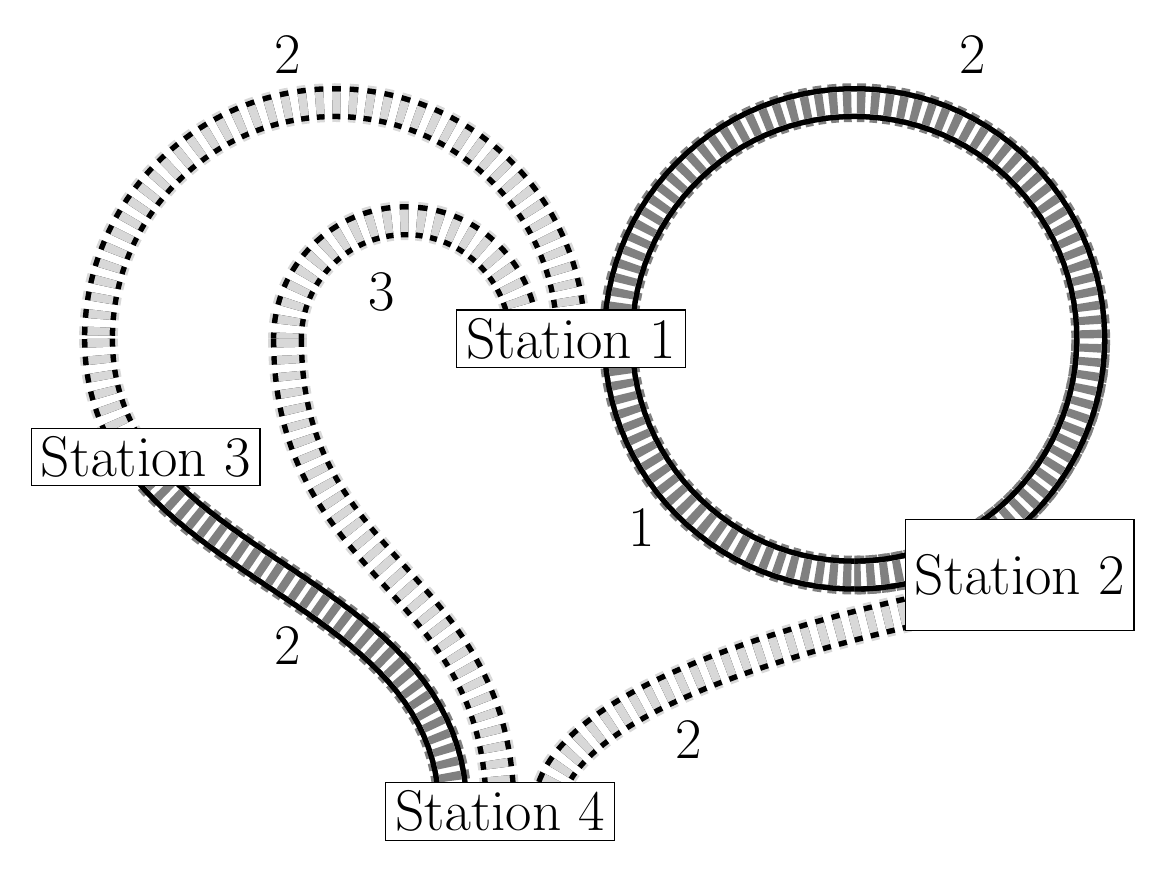
\begin{tikzpicture}[
scale=3
]
%circle 1 and 2
\arcThroughThreePoints[track]{0,0}{1,-1}{2,0};
\arcThroughThreePoints[track]{0,0}{1,1}{1,-1};
%path from 1 to 3
\begin{scope}[shift={(-0.2,0)}]
\clip (-2.3,1.2) rectangle (0.5,-0.5);
\arcThroughThreePoints[dashtrack]{0,0}{-1,1}{-2,0};
\path[dashtrack] (-2,0) .. controls (-2,-1) and (-0.5,-1) .. (-0.5,-2);
\end{scope}
%path from 3 to 4
\begin{scope}[shift={(-0.2,0)}]
\clip (-2.3,-0.5) rectangle (0.5,-2);
\path[track] (-2,0) .. controls (-2,-1) and (-0.5,-1) .. (-0.5,-2);
\end{scope}
%path from 1 to 4
\begin{scope}[shift={(-0.4,0)}]
\arcThroughThreePoints[dashtrack]{0,0}{-0.5,0.5}{-1,0};
\path[dashtrack] (-1,0) .. controls (-1,-1) and (-0.1,-1) .. (-0.1,-2);
\end{scope}
%path from 2 to 4
\path[dashtrack] (1.5,-1.1) .. controls (1,-1.2) and (-0.3,-1.5) .. (-0.3,-2);
%stations
\node[draw,fill=white,anchor=center] at (-0.2,0) {\huge Station 1};
\node[draw,fill=white,anchor=center,minimum height=4em] at (1.7,-1) {\huge Station 2};
\node[draw,fill=white,anchor=center] at (-2,-0.5) {\huge Station 3};
\node[draw,fill=white,anchor=center] at (-0.5,-2) {\huge Station 4};
\node at (1.5,1.2) {\huge 2};
\node at (0.1,-0.8) {\huge 1};
\node at (-1.4,1.2) {\huge 2};
\node at (-1,0.2) {\huge 3};
\node at (-1.4,-1.3) {\huge 2};
\node at (0.3,-1.7) {\huge 2};
\end{tikzpicture}

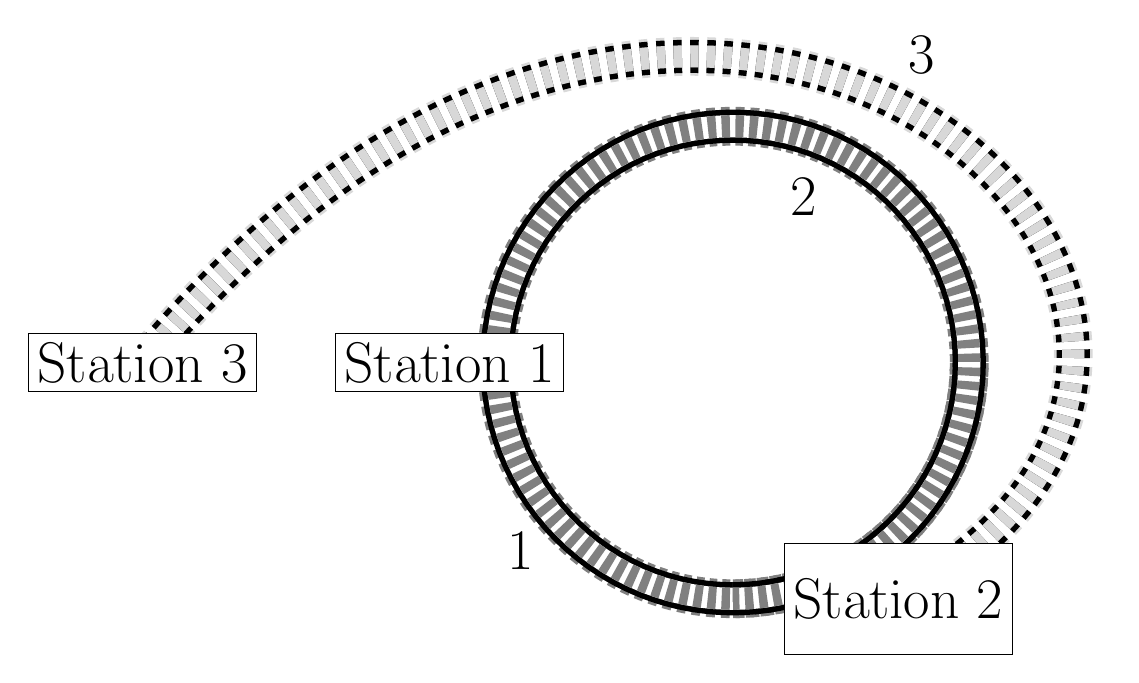
\begin{tikzpicture}[
scale=3
]
%circle 1 and 2
\arcThroughThreePoints[track]{0,0}{1,-1}{2,0};
\arcThroughThreePoints[track]{0,0}{1,1}{1,-1};
%path from 2 to 3
\begin{scope}
\clip  (-1.6,1.4) rectangle (2.6,-1.1);
\path[dashtrack] (1.5,-1.1) .. controls (4,0) and (1,3) .. (-1.5,0);
\end{scope}
%stations
\node[draw,fill=white,anchor=center] at (-0.2,0) {\huge Station 1};
\node[draw,fill=white,anchor=center,minimum height=4em] at (1.7,-1) {\huge Station 2};
\node[draw,fill=white,anchor=center] at (-1.5,0) {\huge Station 3};
\node at (1.3,0.7) {\huge 2};
\node at (0.1,-0.8) {\huge 1};
\node at (1.8,1.3) {\huge 3};
\end{tikzpicture}


\end{document}